\section{Appendix I: Simulation tools}

The simulation tools play a critical role in simulating the background
environment, optimizing the detector setup, and developing the trigger 
and reconstruction strategies. We use GEANT4 and EGS5 to simulate 
electromagnetic interactions. There is generally good agreement 
between these two codes. In particular, no inconsistencies have been 
found on secondary particle yields or energy spectra. However, we have found 
significant disagreements on the angular distributions in the multiple
scattering, bremsstrahlung and pair production processes.  

\vspace{1cm}
\noindent
{\bf Multiple Scattering}

EGS5 simulates the electron elastic scattering using the Moli\`{e}re theory 
\cite{moliere} as formulated by Bethe. \cite{bethe}
It is based on a small angle approximation
($\theta \ll$ 1 radian), and the angular distribution approaches asymptotically
to Gaussian at small angles, and to Rutherford's Coulomb scattering function at 
large angles given by, 

$$ F(\theta) \sim  { 1 \over {(1-cos\theta + {\chi^2 \over 2})^2}}.    \hspace{2 cm} (1) $$

Instead of using the complex and time consuming Moli\`{e}re's formula,
GEANT4 uses two functions explicitly, Gaussian at small angles and the
Rutherford function Eq. (1) at large angles with a requirement that these two
functions and their first derivatives are joined continuously. 
GEANT4, however, uses a different power
in the denominator in Eq. (1) which is close to 2 but not exactly equal to 2 and is 
dependent on the target material and thickness.

Several comparisons have been made in the angular distribution $F(\theta)$ in the
differential cross section $d\sigma=F(\theta)d(cos\theta) d\phi$ for 2.2 GeV electron
scattering from 0.125\% $X_0$ Tungsten target. 
The EGS5 simulation is compared with Moli\`{e}re's analytical formula 
in Figure \ref{appendix:1}(a), demonstrating a good agreement between EGS5 and
the Moli\`{e}re theory.
While the Moli\`{e}re theory is based on a small angle approximation,
the multiple scattering theory developed by Gaudsmit and Saunderson is valid 
for any angle by means of an expansion in Legendre polynomials. \cite{gs}
The validity of the small angle approximation is checked by comparing the 
Moli\`{e}re integral with 
the Goudsmit-Saunderson theory as shown in Figure \ref{appendix:1}(b),
demonstrating that the Moli\`{e}re theory is accurate in the angular region
of the HPS detector. 

\begin{figure*}[h]
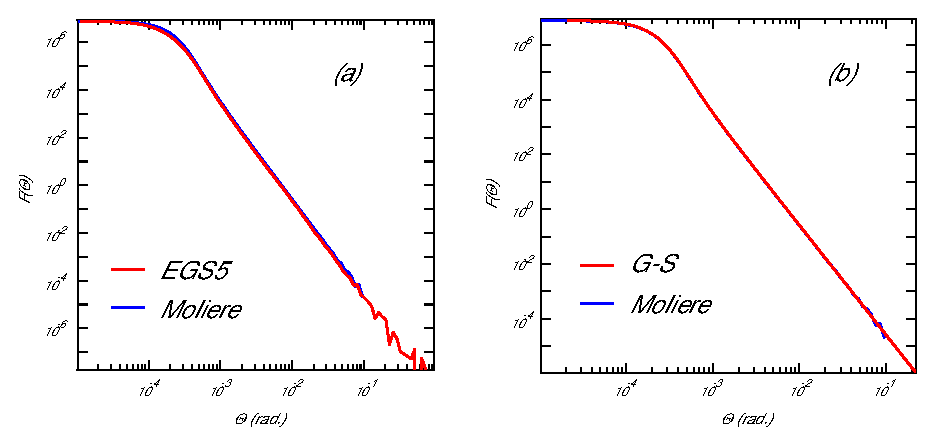
\includegraphics[height=3 in]{appendix/appendix_1.eps}
\caption{\small{ (a) Moli\`{e}re vs. EGS5 \hspace{1 cm} (b) Moli\`{e}re vs. Goudsmit-Saunderson}}
\label{appendix:1}
\end{figure*}

Figure \ref{appendix:2} shows the angular distribution comparison between the GEANT4 
simulation and the Moli\`{e}re integral. 
GEANT4 is in good agreement with the Moli\`{e}re integral up to about 1 mrad, then it 
deviates at larger angles, predicting roughly twice the cross section at 15 mrad, 
where the HPS tracker sensor edge is located.

D. Attwood \etal~ measured 170 MeV muon angular distributions and compared with 
GEANT4 simulations and the Moli\`{e}re theory. \cite{attwood} They concluded that GEANT4 
simulation over-estimated the scattering tail by about a factor of two, and the data were consistent
with the Moli\`{e}re theory. G. Shen \etal~ \cite{shen} and B. Gottschalk \etal~ \cite{gottschalk}
also showed that the Moli\`{e}re theory was consistent with the measurements on a wide variety of
target materials.

\begin{figure}[h]
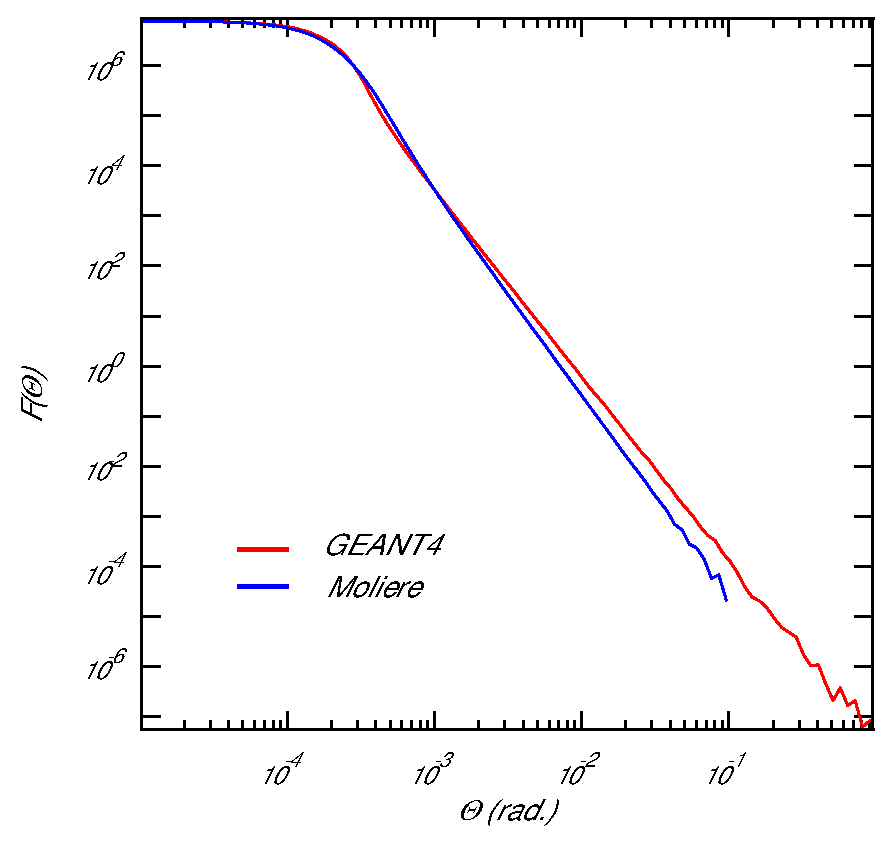
\includegraphics[height= 3 in]{appendix/appendix_2.eps}
\caption{\small{ Moli\`{e}re vs. GEANT4 }}
\label{appendix:2}
\end{figure}

\vspace{1cm}
\noindent
{\bf Angular distributions in the bremsstrahlung and pair production processes}

While GEANT4 and EGS5 are in good agreement in the production rates and the secondary particle
energy spectra, there are significant differences in the angular distribution in the secondary
particles. In EGS5, the angular distributions are sampled from the following differential
cross section for the bremsstrahlung process, \cite{koch}

$$d\sigma(k,\theta_\gamma) = {{4Z^2r_0^2} \over 137} {dk \over k} ydy\{{{16y^2E} \over 
{(y^2+1)^4E_0}}
 -{{(E_0+E)^2} \over {(y^2+1)^2E_0^2}}+\{{{E_0^2+E^2} \over {(y^2+1)^2E_0^2}} -
 {{4y^2E} \over {(y^2+1)^4E_0}}\} lnM(y) \}, $$

\noindent
where $k$ photon energy, $\theta_\gamma$ photon polar angle, $E_0$ and $E$ are initial and final 
electron energy, and

$$y=E_0\theta_\gamma; {1 \over {M(y)}} = ({k \over {2E_0E}})^2 + ({{Z^{1/3}} \over {111(y^2+1)}})^2, $$

\noindent
and for the pair production process, \cite{motz}

$${{d\sigma} \over {dE_\pm d\Omega_\pm}} = {{2\alpha Z^2r_0^2} \over \pi} {E_\pm^2 \over k^3}
\{-{{(E_+-E_-)^2} \over {(u^2+1)^2}}-{{16u^2E_+E_-} \over {(u^2+1)^4}} + \{ {{E_+^2+E_-^2} \over
{(u^2+1)^2}} + {{4u^2E_+E_-} \over {(u^2+1)^4}} \} lnM(u)\},$$

\noindent
where $k$ photon energy, $E_\pm$ $e^{\pm}$ energy, $\theta_\pm$ $e^{\pm}$ polar angle, and

$$u=E_\pm\theta_\pm; {1 \over {M(u)}} = ({k \over {2E_+E_-}})^2+({Z^{1/3} \over {111(u^2+1)}})^2.$$

\noindent
GEANT4 uses an approximate function to simulate the angular distributions in the 
bremsstrahlung and pair production processes given by

$$ f(u) = C [ue^{-au} + d u e^{-3au}], $$

\noindent
with $u=E_0\theta_\gamma$ for incident electron energy $E_0$ and the polar angle 
$\theta_\gamma$ of the bremsstrahlung photon, and $u=E_{\pm}\theta_{\pm}$ for the pair 
energy $E_\pm$ and polar angle $\theta_\pm$ in the pair production. Since the production angle
is typically $1/\gamma$, GEANT4's approximations are acceptable
for most of the high energy detector simulations. However, GEANT4
simulations are inconsistent with the data in the following two cases in the HPS Test Run,

1) GEANT4 prediction on the bremsstrahlung photon angular distribution is too narrow, 
resulting in too few collimator scattering, and

2) GEANT4 prediction on the pair angular distribution is too narrow, resulting in 
too few Ecal trigger rates.

\vspace{1cm}
\noindent
{\bf Conclusions}

Because of these inaccuracies in GEANT4 the electromagnetic interactions in the target are simulated 
by EGS5, and all the particles that come out of the target are passed on to the HPS detector 
simulation system based on GEANT4.

\bibliographystyle{unsrt}
\begin{thebibliography}{99}
\bibitem{moliere}
G. Moli\'{e}re, Z. Naturforsch. {\bf 3a}, 78 (1948)

\bibitem{bethe}
H. A. Bethe, Phys. Rev. {\bf 89}, 1256 (1953)
\bibitem{gs}
S. A. Goudsmit and J. L. Saunderson, Phys. Rev. {\bf 57}, 24 and {\bf 58}, 36 (1940);
K. Okei and T. Nakatsuka, Proceedings of the $17^{th}$ EGS User's Meeting.

\bibitem{attwood}
D. Attwood \etal, Nucl. Instrum. Methods {\bf B251}, 41 (2006)

\bibitem{shen}
G. Shen \etal, Phys. Rev. {\bf 20}, 1584 (1979)

\bibitem{gottschalk}
B. Gottschalk \etal, Nucl. Instrum. Meth. {\bf B74}, 467 (1993)

\bibitem{koch}
H.W. Koch and J.W. Motz, Rev. Mod. Phys. {\bf 31}, 920 (1959)

\bibitem{motz}
J.W. Motz, H. A. Olsen, and H.W. Koch, Rev. Mod. Phys. {\bf 41}, 581 (1969)

\end{thebibliography}
